% Chapter Template

\chapter{Research 10P} % Main chapter title

\label{Chapter2} % Change X to a consecutive number; for referencing this chapter elsewhere, use \ref{ChapterX}

%General explanation: We have an escape room that is currently a WSN with only little data processing, we watn to extend the middleware
% to achieve a broader spectrum of integration possibilities.
As explained in \ref{Chapter1}, the goal of this project was to extend the existing project.
Therefore, we researched possible architectures and practices to integrate to the project.
In the following, research concerning the development of our project is listed and explained.

\section{Design thinking}
Design thinking is one strategy to plan an innovation process. 
It seemed to fit our working process and was a guide concerning our production phase, further explained in \ref{Chapter4}.
In contrast to mechanical improvements, design thinking tries to emphatize with possible customer needs at all parts of the product.
A few of Design thinking's key principles are to 
"engage in early exploration of selected ideas, rapidly modelling potential solutions to encourage learning 
while doing, and allow for gaining additional insight into the viability of 
solutions before too much time or money has been spent" and that it 
"Iterates through the various stages, revisiting empathetic frames of mind and then redefining the challenge as new knowledge and insight is gained along the way." 
\parencite{designThinking}
The Stanford Design School, now known as the Hasso Plattner Institute of Design began teaching a design thinking process 
with the thre steps of understanding, improving and applying a product. 

Since then, their approach to design thinking moved on to a widely used, open-sourced 5 stage process \parencite{designThinkingCrashCourse}
consisting of the following items:
\begin{itemize}
    \item [Empathise]
    Emphatizing relies on three principles: Observe, engage and immerse with your customers
    \item [Define]
    Stanford recommends to unpack the priorly collected findings "to needs and insights and scope a meaningful challenge \parencite{designThinkingBootleg}
    \item [Ideate]
    Ideation is the stage one should explore ideas in a "wide open" \parencite{designThinkingBootleg}. The goal is to create ideas that some 
    can be picked from to create a prototype.
    \item [Prototype]
    Apart from testing, prototyping for this definition of the design thinking process serves many purposes. 
    According to \parencite{designThinkingBootleg}, one can also profit from prototyping for
    \begin{itemize}
        \item Empathy
        \item Exploration
        \item Inspiration
        \item Testing
    \end{itemize}
    purposes. One can receive a deepend understanding by building a prototype (Empathy), explore multiple concepts faster (Exploration),
    inspire other people for one's ideas (Inspiration) test and refine (Testing). 
    Empathy gaining.
    \item [Test]
    The testing is an iterative process where one can refine and gather feedback about the product.
\end{itemize}
Figure \ref{fig:designThinking} illustrates the iterative properties of this model.

\begin{figure}[th]
	\centering
	\includegraphics[width=75mm,scale=0.75]{Figures/designThinking}
	\decoRule
	\caption[designThinking]{Author/Copyright holder: Teo Yu Siang and Interaction Design Foundation. Copyright terms and licence: CC BY-NC-SA 3.0}
	\label{fig:designThinking}
\end{figure}

The model goes on to describe user analyzing methods which are not relevant in the context of this project.

\section{Prototyping (1-2p)}
A prototype is "An initial model of an object built to test a design." \parencite{prototypeDef}
Basic vocabulary will be explained in this section for following chapters.

\subsection{Proof of Concept}
\subsection{Minimal Viable Product}
\subsection{Rapid Prototyping}


\section{Architecture (2-3p)}
//IoT-system, architectures, layers, models, fog/cloud computing //Sensors, actuators

As there is, at this point in time, no consensus reached for a layer model defined for IoT-architectures \parencite{noModel}
different approaches can be used to analyze and structure an IoT-system. 
The following describes three proposed layer-models.

\subsection{Five-Layer architecture}
One by \parencite{fiveLayer1,fiveLayer} proposed model is a five-layer-model consisting of the following layers.
\begin{description}
    \item [Perception layer]
    The perception layer is the physical layer of the architecture. Sensors and actuators exist in this layer.
    \item [Transport layer]
     The transport layer transports data from the perception layer to the processing layer. Different network protocols can be used
   \item [Processing layer]
   The processing layer stores, analyzes and channels incoming data. It is also known as the middleware layer.
   \item [Application layer]
   The application layer is responsible for delivering user-relevant data to a user.
   \item [Business layer]
   The business layer manages the whole system, e.g. applications, business and profit models.
\end{description}

When talking about IoT-architectures, one should mention the difference between cloud and fog/edge based architectures. 
Cloud based architectures assume that processing and analyzing of data should happen in an enviroment remote from the devices' location.
The network below sends data to the cloud, and above the cloud lie applications working with the processed data with the cloud in the center of this architecture.
In the last years, cloud computing has gained popularity, also in the context of IoT architecture \parencite{CloudComputing} because it provides great exibility and scalability.
A newer trend instead are fog or edge based architectures, where the sensors and gateways do parts of the data processing and analytics.
A fog architecture \parencite{FogComputing1, FogComp} presents a layered approach, inserting various layers between the physical (perception) and transport layers 
(monitoring, pre-processing, storage, security). 
Wheras fog computing refers to smart sensors and gateways, edge computing refers to not-smart objects like motors, pumps with 
smart data preprocessing capabilities \parencite{edgeFog}


\begin{figure}[th]
	\centering
	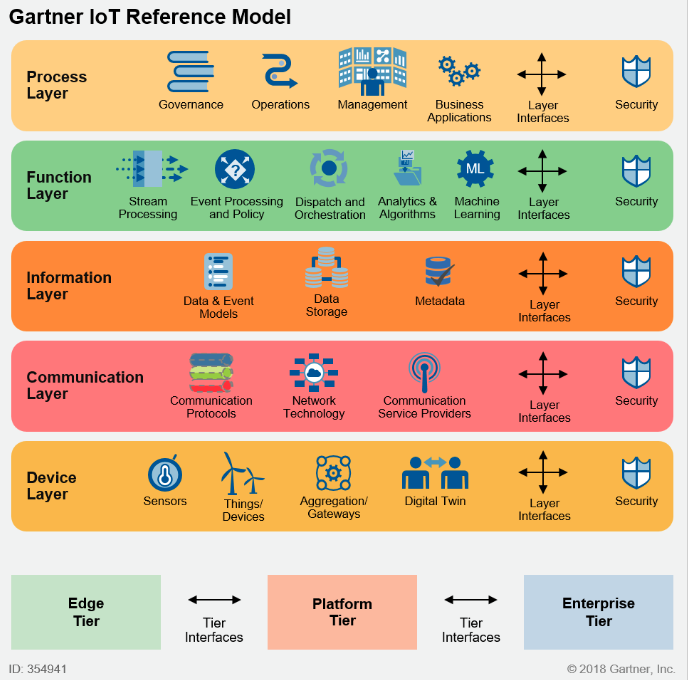
\includegraphics[width=75mm,scale=0.75]{Figures/gartnerIoT}
	\decoRule
	\caption[Gartner]{gartnerIoT1}
	\label{fig:gartnerIoT}
\end{figure}

\section{Communication Protocols}
The project didn't allow changing the communication protocol without disrupting the existing enviroment. 
For future implementations, other communication protocols could be considered for enviroments like this (small room, fast transport).
\subsection{W-LAN}
\subsection{WPan6}
\subsection{ZigBee}
\subsection{MQTT}

\section{Front-End}
As \parencite{frontend} states:
"A front-end system is part of an information system that is directly accessed and interacted with by the user to receive or 
utilize back-end capabilities of the host system. 
It enables users to access and request the features and services of the underlying information system."  

The front-end is the visual component of any application. Disciplines like UX (User Experience), UI(User Interface) and  IxD (Interaction design) have been working on creating 
a "better" front-end-experience for many years. Usually, a mixture of HTML, CSS and javascript is used for front-end development. 
In recent years, libaries that combine HTML and Javascript capabilities like React.js, Angular or Vue %\parencite{reactjsAngularVue} 
have been designed to support a component based architecture. 

For this project, we used React.js.

Reactjs is an Open-Source Javascript-Libary.
After developing Reactjs in 2011, Facebook soon discovered that it's performance was faster than other implementations of its' kind and made it Open-Source in 2015. 
At present, React is used by major companies for their front-end like Airbnb, Netflix and Reddit \parencite{reactjsUsers}. 
In this years' Stackoverflow-Survey, React came third in "Most Popular Framework, libary or Tool" \parencite{stackOverflowSurvey}. 
This year, over 100,000 developers participated in the survey. 
A lot of libaries are available for react. 
Its main concepts are:
\begin{description}
    \item[Components] \hfill \\
    React motivates its' users to write encapsulated components with single responsibilities. Components combine the HTMl-markup and Javscript-functionality of a responsibility. They are supposed to reusability. %erhöhen
    \item[Composition] \hfill \\
    The user can reuse and composite elements as he needs to. The isolated components makes code easier to maintain. 
    \item[Uni-Directional Dataflow] \hfill \\
            Properties should not be changed in other components, but passed down as read-only variables. 
            React doesn't want children to affect their parent components. That makes maintainability easier, as there's a clear downward structure in a well designed React project.
            If a user needs to pass changes to a parent component, it's executed with callbacks, or, for more complicated architecture with a Flux-supporting libary like Redux.
    \item[Virtual Dom]\hfill \\
    A DOM%Reference to Abkürzung 
    is a logical structure of documents in HTML, XHTML, or XML formats. 
    Web browsers are using layout engines to transform or parse the representation HTML-syntax into document object model that we can see in a web browser.
    Usually, when one of these elements changes, the whole structure has to be calculated again. 
    React uses a Virtual DOM as a negiator to enable calculating only the parts that need calculating. That's also possible because of Reacts' isolated component structure.
    \item[JSX]  JSX, short for Javascript XML, is an implementation of Javascript which is usually used to write in ReactJs. 
    It looks a lot like HTML but enables Javascript functionality. Javascript functionalities can be used by putting them in curly brackets ("{}").
\end{description}

\section{Communication}
%Socket.io
There are different ways to communicate between clients and middleware. 
Communication on the web is usually unsynchronized. 
The client requests and the server responds. 
Problems arise if real-time communication is required. 
Chat-Applications shouldn't require the user to reload a page anytime he wants to see a new message.
Those services demand a more reactive and immediate communication.

For this, web development techniques like AJAX \parencite{ajax} were invented. 
Here, the client requests data automatically, establishing a new connection to the server.

This technique needs a client to request new content instead of listening 
for new information which creates unnessecary overhead and a higher latency than other communication enviroments like WebSockets.  
 
WebSockets pursue this task by creating a bilateral environment for clint-server-exchange. 
This way, the client doesn't need to connect again and again, but listens for events. 
Now-a-days, most browsers are Websocket compatible.

For this project, Socket.io was used for client-middleware-communication.

Socket.io is a Javascript-Libary designed for realtime communication build on top of a websocket-protocol.
It enables a bi-directional communication channel between client and server and offers a fallback mechanism to long polling when WebSockets are not available.
There are several fallback mechanisms available that are determined dynamically by Socket.io:
\begin{itemize}
    \item WebSocket
    \item Adobe Flash Socket
    \item AJAX long polling
    \item AJAX multipart streaming
    \item Forever Iframe
    \item JSONP Polling
\end{itemize}

The server-side of Socket.io is developed  specifically for Node.js wheras for the client different implementations (e.g. .Net, Swift, C++)\parencite{socketioClients} are available.
Once a connections is established it's maintained and uses a diminishing small amount resources to communicate. 
It uses an event-based system where one participant listens and another emits an event. 
Both Client and Server can emit and listen for events.

\section{Middleware}
%Talk about Node.js
//Was ist middleware? in dme fall node js
Node.js is an open-source, cross-plattform, javascript-runtime-enviroment. 
With 49.6\% it is this years "Most Popular Framework, Libary or Tool" on this years Stackoverflow-survey \parencite{stackOverflowSurvey}.
According to Google Trends, interest is rising since 2012\parencite{gogleTrendNode}.
One explanation for that might be that it's written in Javascript. 
The transation for front-end Javascript developers to developing back-end is eased, which saves companies learning costs.
Node.js is estimated to have a high learning curve \parencite{nodeLearningcurve}.
It uses an event-driven architecture which operates on a single threaded event loop using non-blocking I/O calls.
Commands use callbacks to signal they are completed or failed. 
A downside is, that it doesn't allow vertical scaling by increasing the number of CPU cores of the machine it is running on. 
On CPU-intensive applications, that might become a problem - but modules like IPC or pm2 can add that functionality.
Node.Js commands are non-blocking and execute concurrently or in parallel. 
It's build on the Google V8 JavaScript engine which compiles Javascript to machine code instead of interpreting it in real time. 
That makes it faster than (some) other engines.
There are thousands of open-source libaries and web frameworks available for Node.js. 
\section{Device}
%Talk about Arduino implementation
//Was ist ein device im iot kontext? die microcontroller 
Arduino is a microcontroller-company from italy which was founded in 2005. 
It is completely open source and provides its own Integrated Development Enviroment(IDE) \parencite{arduinoIDEDownload}.
The IDE works with nearly all microprocessors on the market. 
The IDE recommends a structure for all Arduino programs:
\begin{description}
    \item [Initialization]
    Prior to any function, libaries and necessary variables are declared within an Arduino program.
    \item [setup()]
    The setup-function is the first function called in any Arduino-program.
    \item [loop()]
\end{description}
The Arduino (and comperable microprocessors) are programmed in C.
\section{Back-End}
%Talk about postgres
//Back end was ist das in diesem fall wurde das benutzt
Postgres is a light-weight open-source object-relational database system. 
Companies like Netflix, Spotify or Instagram \parencite{postgresUsers} rely on the flexible database system which allows SQl and noSQL design.
It is easy to set-up and maintain. 


%Even though, only 26\% of IoT-Projects in companies are judged to be a complete success 
%\parencite{ciscoresearch}. The reasons are as numerous as they are diverse. 
%Lack of knowledge, lack of planning, inconsistent standards and legacy architectures within the project are only some mentioned by the Cisco survey.
%A McKinsey report \parencite{mcKinsey} in 2015 stated that most IoT adopters fail to use their data or derive just a small part of its value.
